\documentclass[journal]{IEEEtran}
%
% General
%
\usepackage[english]{babel}

%
% Graphics
%
\usepackage{graphicx}

%
% Shortcuts
%
\newcommand{\up}[1]{#1}

\newcommand{\rv}{random variable}
\newcommand{\rvs}{random variables}
\newcommand{\perse}{\emph{perse}}

%
% References
%
\newcommand{\aref}[1]{Algorithm~\ref{alg:#1}}
\newcommand{\eref}[1]{(\ref{equ:#1})}
\newcommand{\fref}[1]{Fig.~\ref{fig:#1}}
\newcommand{\rref}[1]{Remark~\ref{rem:#1}}
\newcommand{\sref}[1]{Sec.~\ref{sec:#1}}

\newcommand{\alab}[1]{\label{alg:#1}}
\newcommand{\elab}[1]{\label{equ:#1}}
\newcommand{\flab}[1]{\label{fig:#1}}
\newcommand{\rlab}[1]{\label{rem:#1}}
\newcommand{\slab}[1]{\label{sec:#1}}

%
% Formatting
%
\usepackage{lettrine}
\usepackage[factor=1700]{microtype}
\newcommand{\subscript}[1]{\text{\kern0.1em#1}}

\setlength{\textfloatsep}{10pt}
\setlength{\parskip}{0pt}

\setlength{\abovedisplayskip}{4pt}
\setlength{\belowdisplayskip}{4pt}

\raggedbottom
\clubpenalty 0
\widowpenalty 0
\predisplaypenalty 0
\postdisplaypenalty 0

\makeatletter
\let\origsection\section
\renewcommand\section{\@ifstar{\starsection}{\nostarsection}}
\newcommand\nostarsection[1]
{\sectionprelude\origsection{#1}\sectionpostlude}
\newcommand\starsection[1]
{\sectionprelude\origsection*{#1}\sectionpostlude}
\newcommand\sectionprelude{%
  \vspace{-0.3em}
}
\newcommand\sectionpostlude{%
  \vspace{-0.1em}
}
\makeatother

\usepackage{hyperref}

%
% Algorithms
%
\usepackage{algorithm}
\usepackage{algpseudocode}

% To make algorithms float
\usepackage{float}
\newfloat{algorithm}{t}{lop}

% To have aligned comments
\usepackage{eqparbox}
\renewcommand{\algorithmiccomment}[1]{\hfill\eqparbox{COMMENT}{// #1}}

\newcommand*\Let[2]{\State #1 = #2}
\renewcommand{\algorithmicrequire}{\textbf{Input:}}
\renewcommand{\algorithmicensure}{\textbf{Output:}}

\renewcommand*\ttdefault{cmtt}
\usepackage[T1]{fontenc}
\newcommand{\token}[1]{\texttt{#1}}

\newenvironment{compactlist}{
  \begin{list}{}{
    \setlength\partopsep{0pt}
    \setlength\parskip{0pt}
    \setlength\parsep{0pt}
    \setlength\topsep{0pt}
    \setlength\itemsep{0pt}
    \setlength{\itemindent}{1em}
    \setlength{\leftmargin}{0pt}
  }
}{
  \end{list}
}

\newcommand{\point}[1]{\item\emph{#1}}

%
% Mathematics
%
\usepackage{amsmath}
\usepackage{amssymb}
\usepackage{bm}
\usepackage{dsfont}
\usepackage{cases}

\usepackage{amsthm}
\newtheorem{remark}{Remark}

\newcommand{\error}{\epsilon}

% Real analysis and functional analysis
\newcommand{\real}{\mathbb{R}}
\newcommand{\continuous}{\mathcal{C}}

\newcommand{\norm}[1]{\| #1 \|}
\newcommand{\card}[1]{\left| #1 \right|}

% Linear algebra
\newcommand{\m}[1]{\mathbf{#1}}
\renewcommand{\v}[1]{\mathbf{#1}}
\newcommand{\diag}{\text{diag}}

% Interpolation
\newcommand{\f}{f}

\newcommand{\tensor}[1]{\mathcal{Q}_{#1}}
\newcommand{\smolyak}[1]{\mathcal{S}_{#1}}
\newcommand{\approximation}[1]{\mathcal{A}_{#1}}

\newcommand{\lindex}{\mathcal{I}}
\newcommand{\oindex}{\mathcal{J}}

\renewcommand{\l}{l}

\newcommand{\vi}{\v{i}}
\newcommand{\vj}{\v{j}}
\newcommand{\vl}{{\bm{\iota}}}

\newcommand{\e}{e}
\newcommand{\E}{\mathcal{E}}

\newcommand{\w}{v}

\newcommand{\x}{x}
\newcommand{\vx}{\v{x}}
\newcommand{\X}{\mathcal{X}}

\newcommand{\Y}{\mathcal{Y}}

\newcommand{\Z}{\mathcal{Z}}

\newcommand{\surplus}{\Delta\f}
\newcommand{\score}{s}

\newcommand{\aerror}{\error_a}
\newcommand{\rerror}{\error_r}
\newcommand{\serror}{\error_s}

% Probability theory
\newcommand{\outcomes}{\Omega}
\newcommand{\sigmaAlgebra}{\mathcal{F}}
\newcommand{\probabilityMeasure}{\mathbb{P}}
\newcommand{\probabilitySpace}{(\outcomes, \sigmaAlgebra, \probabilityMeasure)}

\renewcommand{\o}{\omega}

\newcommand{\distribution}{F}
\newcommand{\correlation}{\m{R}}

\newcommand{\expectation}[1]{\mathbb{E} \, #1}
\newcommand{\variance}[1]{\mathbb{V}\text{ar} \, #1}

\newcommand{\h}{\xi}
\newcommand{\vh}{\bm{\xi}}

\newcommand{\transformation}{\mathbb{T}}

%
% Platform and application
%
\renewcommand{\b}{b}
\newcommand{\vb}{\v{\b}}

\renewcommand{\d}{d}
\newcommand{\vd}{\v{\d}}

%
% Time
%
\newcommand{\ts}{\mathrm{T}}
\renewcommand{\t}{t}

%
% Power
%
\newcommand{\p}{p}
\newcommand{\vp}{\v{\p}}
\newcommand{\mP}{\m{P}}

\newcommand{\dynamic}{\subscript{d}}
\newcommand{\static}{\subscript{s}}

%
% Temperature
%
\newcommand{\mC}{\m{C}}
\newcommand{\mG}{\m{G}}

\newcommand{\vs}{\v{s}}

\newcommand{\q}{q}
\newcommand{\vq}{\v{\q}}
\newcommand{\mQ}{\m{Q}}

\newcommand{\mM}{\m{M}}

\newcommand{\ambient}{\subscript{amb}}

%
% Uncertain parameters
%
\renewcommand{\u}{u}
\newcommand{\vu}{\v{u}}

\newcommand{\z}{z}
\newcommand{\vz}{\v{z}}

\newcommand{\g}{g}

%
% Numbers
%
\newcommand{\n}{n}

\renewcommand{\nu}{{\n_\u}}
\newcommand{\nz}{{\n_\z}}
\newcommand{\np}{{\n_\pi}}
\newcommand{\nt}{{\n_t}}
\newcommand{\ns}{{\n_\t}}
\newcommand{\nn}{{\n_\text{n}}}
\newcommand{\nin}{{\n_\text{d}}}


\title{
  Probabilistic Analysis of Electronic Systems\\
  via Adaptive Hierarchical Interpolation
}
\author{Ivan Ukhov,
Petru Eles,~\IEEEmembership{Member,~\up{IEEE}}, and
Zebo Peng,~\IEEEmembership{Senior Member,~\up{IEEE}}
\vspace{-2.5em}
\thanks{
  The manuscript was received on July 15, 2016, revised on November 17, 2016,
  and on February 3, 2017, and accepted on April 14, 2017.
}%
\thanks{
  The authors are with the Department of Computer and Information Science,
  Link\"{o}ping University, SE-581\,83 Link\"{o}ping, Sweden (e-mails:
  ivan.ukhov@liu.se, petru.eles@liu.se, and zebo.peng@liu.se, respectively).
}%
\thanks{
  Digital Object Identifier XX.XXXX/TCAD.XXXX.XXXXXXX
}%
}

\begin{document}
  \maketitle

  \begin{abstract}
    We present a design-time system-level framework for the analysis of electronic
systems whose runtime behavior dependents on uncertain parameters. The proposed
approach thrives on adaptive hierarchical interpolation, which makes it general
and suitable for studying various quantities that are of interest to the
designer. Examples of such quantities include the end-to-end delay, total energy
consumption, and maximal temperature of the system under consideration. The
framework delivers a light generative model and allows for a straightforward,
computationally efficient calculation of the probability distribution and
accompanying statistics of the quantity of interest. Our technique is
illustrated by considering a number of applications and comparing the
corresponding results, in terms of both speed and accuracy, with exhaustive
computer simulations.

  \end{abstract}

  \begin{IEEEkeywords}
    Hierarchical interpolation,
    local adaptivity,
    probabilistic analysis,
    sparse grids,
    uncertainty quantification.
  \end{IEEEkeywords}

  \bstctlcite{IEEEexample:BSTcontrol}

  \section{Introduction} \slab{introduction}
  The work is based on work in \cite{klimke2006} and \cite{ma2009}.

The approach belongs to the class of stochastic collocation techniques
\cite{xiu2010}. The major distinctive feature of stochastic collocation is the
usage of interpolation as a means of uncertainty quantification, which should be
contrasted with other techniques such as polynomial chaos expansions relying on
regression. The application of popular polynomial expansions is limited in this
case due to the non-smoothness of the response surface.

The remainder of the paper is organized as follows.


  \section{Prior Work} \slab{prior-work}
  Computer experiments together with Monte Carlo (\abbr{MC}) methods would be a
reasonable solution to probabilistic analysis of electronic systems if
electronic systems were inexpensive to simulate (in terms of time, money, or
other resources). In order to eliminate or reduce the costs associated with
direct sampling, a number of techniques have been introduced. The techniques are
diverse as the area itself and can be classified in many ways. Two natural
characteristics, distinguishing the techniques, originate from the sources of
uncertainty and quantities of interests that the techniques have been tailored
for. A technique tries to give a probabilistic characterization of the latter
while taking into account the deteriorating effect of the former. The solution
that a technique proposes to tackle the corresponding problem is another
characteristic to pay attention to. A solution can be based on, for instance, a
mathematical framework, statistical method, or computational algorithm. In what
follows, we shall focus on the three aforementioned characteristics.

Let us first discuss analog sources of uncertainty and, more concretely, process
variation as it by far dominates. Circuit-level timing and power analyses under
process variation are undertaken in \cite{bhardwaj2008} by means of polynomial
chaos (\abbr{PC}) expansions \cite{xiu2010}. The work in \cite{juan2012} models
static steady-state temperature and accounts for process variation by leveraging
the linearity of Gaussian distributions and time-invariant systems. A stochastic
collocation \cite{xiu2010} approach to static steady-state temperature analysis
is given in \cite{lee2013}, which relies on global interpolation using Newton
polynomials. In \cite{ukhov2014}, transient temperature analysis is considered,
and process variation is address via \abbr{PC} expansions. The machinery of
\abbr{PC} expansions is also utilized in \cite{ukhov2015} in order to model
dynamic steady-state temperature and to enhance reliability models.

Let us now turn to digital sources of uncertainty. In this context, timing
analysis has drawn the major attention \cite{quinton2012}. A seminal work on
response time analysis of periodic tasks with random execution times on
uniprocessors is reported in \cite{diaz2002}. A novel analytical solution to
this problem is given in \cite{tanasa2015}, which makes milder assumptions and
allows for addressing larger, previously infeasible problems. The framework
proposed in \cite{santinelli2011} facilitates task scheduling by providing
probabilistic bounds on the resource given to a task flow and the resource
needed by that task flow; the approach is based on real-time calculus and is
applicable to electronic systems. Temperature variations due to uncertainties in
timing have also been extensively studied, and the accent has been primarily on
the worst case. An example is the work in \cite{yang2013}, which builds on
real-time calculus and targets the maximal temperature.

Studying the literature on probabilistic analysis of electronic systems, one can
note a pronounced trend: the generality and straightforwardness of \abbr{MC}
methods tend to be lost. To elaborate, a technique typically: 1) requires
restrictive conditions to be fulfilled such as the absence of dependencies or
the usage of a certain scheduling policy; 2) is tailored to one concrete
quantity such as the response time or maximal temperature; and 3) requires
substantial effort in order to be deployed. This trend is, of course,
reasonable: the techniques try to excel by narrowing down the scope and asking
for more. However, it is also important to keep in mind what is practical. 1)
Despite making mathematics beautiful, some of the assumptions often do not hold,
and the independence assumption is one of them. 2) Having one tool for one job
might lead to a longer adoption time and to more experts involved. It is a
sustainable strategy, though, as long as tools are composable, compatible with
each other, which might be difficult to achieve when techniques have drastically
different foundations. 3) It is often the case that there has already been
developed a robust simulator of the quantity under consideration for the ideal
deterministic case. Switching gears to probabilistic analysis might mean
discarding this battle-tested code all together and implementing something else
from scratch, which is wasteful and not desirable.

Some of the techniques listed earlier in this section, in fact, preserve the
generality and straightforwardness of \abbr{MC} methods. An example is the
uncertainty analysis presented in \cite{ukhov2015}. The reason is that the
construction of \abbr{PC} expansions in \cite{ukhov2015} is undertaken by means
of so-called nonintrusive spectral projections \cite{xiu2010}, which do not need
to look inside the ``black box,'' similar to \abbr{MC} methods. However, as
motivated in \sref{introduction}, nonsmoothness is a serious problem for global
approximation based on polynomials. The convergence of \abbr{PC} expansions, for
instance, deteriorates substantially in such cases, requiring partitioning of
the stochastic space in order to alleviate the problem. Therefore, it is not
straightforward to apply such techniques as the one given in \cite{ukhov2015} in
the context of digital sources of uncertainty exhibiting nonsmoothness.

To conclude, the available techniques for probabilistic analysis of electronic
systems are restricted in use. Flexible, capable, and easy-to-deploy frameworks
are needed.


  \section{Our Contribution} \slab{present-work}
  Our work brings the following major contribution. We develop an efficient
framework for probabilistic analysis of electronic systems that is
straightforward to use and is applicable to a wide range of
uncertainty-quantification problems.

The usage of our framework is streamlined because it has the same low entrance
requirements as sampling techniques: one only has to be able to evaluate the
quantity of interest given a set of deterministic parameters. Moreover, the
framework can be utilized in scenarios with limited knowledge about the joint
probability distribution of the uncertain parameters, which are common in
practice (to be elaborated on in \sref{parameters}).

The scope of our framework is wide because the framework has a powerful
approximation engine. We make use of adaptive hierarchical interpolation on
sparse grids \cite{jakeman2012, klimke2006, ma2009}, which enable us to tackle
diverse electronic-system-design problems while keeping the associated
computation costs low. In particular, the framework is suitable for nonsmooth
problems, which is an important feature in the context of electronic systems due
to their digital nature, as discussed in \sref{introduction}.

In addition to the aforementioned contribution, we open-source our
implementation \cite{sources}. The implementation is broken down into multiple
standalone libraries, which makes it well disposed to cherry-picked reusage. The
code base also includes the whole experimental setup described in
\sref{experimentation}.


  \section{Preliminaries} \slab{preliminaries}
  Let $\probabilitySpace$ be a probability space where $\outcomes$ is a set of
outcomes, $\sigmaAlgebra \subseteq 2^\outcomes$ is a $\sigma$-algebra, and
$\probabilityMeasure: \sigmaAlgebra \to [0, 1]$ is a probability measure
\cite{durrett2010}. A \rv\ $\h$ defined on $\probabilitySpace$ is an
$\sigmaAlgebra$-measurable function $\h: \outcomes \to \real$. A \rv\ is
uniquely characterized by its distribution function defined by
$\distribution_\h(z) = \probabilityMeasure(\{ \o \in \outcomes: \h(\o) \leq z
\})$, written as $\h \sim \distribution_\h$. The expected value and variance of
$\h$ are given by
\begin{align}
  & \expectation{\h} = \int_\outcomes \h(\o) \, \d\probabilityMeasure(\o) = \int_\real z \, \d\distribution_\h(z) \hspace{1em} \text{and} \elab{expectation} \\
  & \variance{\h} = \expectation{\h^2} - (\expectation{\h})^2,\text{ respectively.} \elab{variance}
\end{align}

A random vector $\vh = (\h_i)_{i = 1}^n$ is a vector whose elements are \rvs. A
random vector is fully characterized by its distribution function
$\distribution_{\vh}$, written as $\vh \sim \distribution_{\vh}$. This function
is referred to as a joint or multivariate distribution function, emphasizing the
fact that the variables work together.

An $n$-variate distribution can be expressed as a set of $n$ marginal
(univariate) distributions and an $n$-dimensional copula \cite{nelsen2006}. The
copula is a uniform distribution function on $[0, 1]^n$ (referred to as the
$n$-dimensional unit hypercube) that captures the dependencies between the $n$
individual variables.


  \section{Problem Formulation} \slab{problem-formulation}
  Consider an electronic system composed of two major components: a platform and
an application. The platform is given a set of heterogeneous processing elements
$\procs = \{ 1, \dots, \np \}$, and the application is given as a set of tasks
$\tasks = \{ 1, \dots, \nt \}$. In what follows, the system will be denoted by
$(\procs, \tasks)$.

The designer is assumed to be interested in studying a quantity $\g$ that
characterizes the system described above. Examples of $\g$ include the
end-to-end delay, total energy, maximal temperature, and power and temperature
profiles. The quantity $\g$, referred to as the quantity of interest, depends on
a set of parameters that are uncertain at the design stage. The uncertain
parameters are modeled by a random vector $\vu = (\u_i)_{i = 1}^\nu$ with
distribution $\distribution_\vu$. Examples of $\vu$ include the execution times
of the tasks. The dependency of $\g$ on $\vu$, written as $\g(\vu)$, inevitably
implies that $\g$ is random to the designer. For a given $\vu$, however, $\g$ is
assumed to be purely deterministic. Furthermore, the evaluation of $\g$ given
$\vu$ is assumed to be doable but computationally or otherwise expensive. If the
cost of $\g$ was negligible, one could proceed to \abbr{MC} methods directly
without involving any auxiliary framework.

Our objective in this paper is to develop an efficient framework for
probabilistic analysis of the quantity of interest $\g$ characterizing the
system $(\procs, \tasks)$ such that the uncertainty originating from the
parameters $\vu$ is taken into consideration. Probabilistic analysis of $\g$
refers to the estimation of the probability distribution of $\g$, which
naturally implies the availability of such quantities as the expected value and
variance of $\g$ and probabilities of arbitrary events associated with $\g$.


  \section{Solution} \slab{solution}
  As noted earlier, making use of an adequate sampling method is a compelling
approach to uncertainty quantification. We would readily apply such a method to
study our quantity of interest $\g$ if only $\g$ had a negligible cost, which it
does not.

Our solution to the above quandary is to construct a light representation of the
heavy $\g$ and study this representation instead of $\g$. The surrogate that we
build is based on adaptive interpolation: $\g$ is evaluated at a number of
strategically chosen collocation nodes, and any other values of $\g$ are
reconstructed on demand (without involving $\g$) using a set of basis functions
mediating between the collected values of $\g$. The benefit of this approach is
in the number of invocations of the quantity of interest $\g$: only a few
evaluations of $\g$ are needed, and the rest of our probabilistic analysis is
powered by the interpolant, which has a negligible cost, in contrast to $\g$.

Let us delineate the steps involved in the solution process. Recall that $\g$ is
parameterized by the uncertain parameters $\vu$, and these variables are the
only source of randomness. First, we reparameterize $\g$ in terms of an
auxiliary random vector $\vz$ extracted from $\vu$; the necessity of this stage
will become clear later on. Second, we construct an interpolant of $\g$ by
considering $\g$ as a deterministic function of $\vz$ and evaluating $\g$ at a
small set of carefully chosen points $\{ \vz_i \}$. Finally, we estimate the
probability distribution of $\g$ by applying an arbitrary sampling method to the
constructed interpolant of $\g$.

Interpolation of multivariate functions is a challenging task, which should be
approached with a great care. This aspect will be discussed in detail in
\sref{interpolation}. However, before we proceed to interpolation, we first need
to substantiate further the uncertain parameters and quantities of interest.


  \section{Modeling} \slab{modeling}
  The agenda for this section is as follows. In \sref{parameters}, the uncertain
parameters $\vu$ are transformed into a form suitable for the subsequent
calculations. This stage is an essential part of our framework. The rest of the
subsections, \sref{time}, \sref{power}, and \sref{temperature}, serve a strictly
educational, illustrative purpose. They introduce a number of models and a
number of quantities of interest $\g$ in order to give the reader a better
intuition about the utility of the framework. These models and quantities also
give us concrete problems to work with in the section on experimental results,
\sref{experimentation}. It should be well understood that the essence of $\g$ is
problem specific. Therefore, the exact formulation of $\g$ is left to the
designer's discretion.

\subsection{Uncertainty Parameters} \slab{parameters}
The foremost step of our framework is to change the parameterization of the
problem from the random vector $\vu = (\u_i)_{i = 1}^\nu \sim \distribution_\vu$
to an auxiliary random vector $\vz = (\z_i)_{i = 1}^\nz \sim \distribution_\vz$
such that: 1) the support of $\distribution_\vz$ is the unit hypercube $[0,
1]^\nz$, and 2) $\nz \leq \nu$ has the smallest value needed to retain the
desired level of accuracy. The first is standardization, which is done primarily
for convenience. The second is model-order reduction, which identifies and
eliminates excessive complexity and, hence, speeds up the solution process. The
reduction is possible whenever there are dependencies between $(\u_i)_{i =
1}^\nu$, in which case one can find such $(\z_i)_{i = 1}^\nz$, $\nz < \nu$, that
each $\u_i$ can be recovered from $(\z_i)_{i = 1}^\nz$. We shall denote the
overall transformation by $\vu = \transformation(\vz)$ where
\begin{equation} \elab{transformation}
  \transformation: \real^\nu \to [0, 1]^\nz.
\end{equation}
For any point $\vz \in [0, 1]^\nz$, we are now able to compute the corresponding
$\vu$ and, consequently, the quantity of interest $\g$ as $(\g \circ
\transformation)(\vz) = \g(\transformation(\vz)) = \g(\vu)$; recall also
\sref{problem}.

Let us consider an example of $\transformation$ in order to understand the
concept better. To this end, we begin by assuming that the distribution of $\vu
= (\u_i)_{i = 1}^\nu$, $\distribution_\vu$, is given as a set of marginal
distribution functions $\{ \distribution_{\u_i} \}_{i = 1}^\nu$ and a copula
\cite{nelsen2006} (see also \sref{preliminaries}). Furthermore, the copula is
assumed to be a Gaussian copula whose correlation matrix is $\correlation \in
\real^{\nu \times \nu}$.

\begin{remark}
A set of marginals and a copula entirely characterize the joint distribution of
$\vu$, that is, $\distribution_\vu$. However, we consider this distribution as
an approximation rather than as the true one. The knowledge of the true joint
would be an impractical assumption to make. A more realistic assumption is the
availability of the marginals and correlation matrix of $\vu$. In general, these
two pieces are not sufficient to recover the joint of $\vu$; however, the joint
can be approximated well by accompanying the available marginals by a Gaussian
copula constructed based on the available correlation matrix; see \cite{liu1986}
and also \cite{ukhov2014}. Hence, a set of marginals and a Gaussian copula are
practical inputs to probabilistic analysis.
\end{remark}

The number of variables, which is so far $\nu$, has a significant impact on the
complexity of the problem at hand. Therefore, an important component of our
framework is model-order reduction, which we shall base on the discrete
Karhunen--Lo\`{e}ve decomposition, also known as the principal component
analysis. We proceed as follows. Since any correlation matrix is real and
symmetric, $\correlation$ admits the eigendecomposition: $\correlation = \m{V}
\m{\Lambda} \m{V}^T$ where $\m{V} \in \real^{\nu \times \nu}$ is an orthogonal
matrix whose columns are the eigenvectors of $\correlation$, and $\m{\Lambda} =
\diag(\lambda_i)_{i = 1}^\nu$ is a diagonal matrix whose diagonal elements are
the eigenvalues of $\correlation$. The eigenvalues $(\lambda_i)_{i = 1}^\nu$
correspond to the variances of the corresponding components revealed by the
decomposition. The model-order reduction boils down to selecting those major
components whose cumulative contributions to the total variance is above a
certain threshold. Formally, assuming that $(\lambda_i)_{i = 1}^\nu$ are sorted
in the descending order and given a threshold $\eta \in (0, 1]$ specifying the
fraction of the total variance to be preserved, we identify the smallest $\nz$
such that
\begin{equation} \elab{reduction}
  \frac{\sum_{i = 1}^\nz \lambda_i}{\sum_{i = 1}^\nu \lambda_i} \geq \eta.
\end{equation}
Denote by $\tilde{\m{V}} \in \real^{\nu \times \nz}$ and $\tilde{\m{\Lambda}}
\in\real^{\nz \times \nz}$ the matrices obtained by truncating $\m{V}$ and
$\m{\Lambda}$, respectively, to preserve only the first $\nz$ components where
$\nz$ is as shown above.

Now, the transformation $\transformation$ in \eref{transformation} is
\begin{equation} \elab{transformation-concrete}
  \vu = \distribution_\vu^{-1} \left( \Phi\left( \tilde{\m{V}} \tilde{\m{\Lambda}}^\frac{1}{2} \, \Phi^{-1}(\vz) \right) \right)
\end{equation}
where the \rvs\ $\vz = (\z_i)_{i = 1}^\nz$ are independent and uniformly
distributed on $[0, 1]^\nz$; $\Phi$ and $\Phi^{-1}$ are the distribution
function of the standard Gaussian distribution and its inverse, respectively,
which are applied elementwise; and $\distribution_\vu^{-1} =
\distribution_{\u_1}^{-1} \times \cdots \times \distribution_{\u_\nz}^{-1}$ is
the Cartesian product of the inverse marginal distributions of $\vu$, which are
applied to the corresponding element of the vector yielded by $\Phi$. In the
absence of correlations, \eref{transformation-concrete} is simply $\vu =
\distribution_\vu^{-1}(\vz)$, and no model-order reduction is possible ($\nu =
\nz$). It might be interesting to note that, using the above transformation, the
distribution $\vu$ gets ``baked'' in $\g$ because it ``disappears'' when $\g$ is
viewed as a function of $\vz$, distributed uniformly.

To summarize, we have found such a transformation $\transformation$ and the
corresponding random vector $\vz \sim \distribution_\vz$ that: 1)
$\distribution_\vz$ is supported by $[0, 1]^\nz$, and 2) $\vz$ has the smallest
number of dimensions $\nz$ needed to preserve $\eta$ portion of the variance.


\subsection{Application Timing} \slab{time}
Suppose the application is given as a directed acyclic graph. The vertices
represent tasks, and the edges data dependency between these tasks. Suppose
further that a static cyclic scheduling policy is utilized. Note, however, these
assumptions are orthogonal to our framework: the framework can be applied to any
application model and any scheduling policy.

Each task has a start and a finish time. For task $i$, denote these two time
moments by $\b_i$ and $\d_i$, respectively, and let $\vb = (\b_i)_{i=1}^\nt$ and
$\vd = (\d_i)_{i=1}^\nt$. Other timing characteristics of the application can be
derived from $(\vb, \vd)$. An example is the end-to-end delay, which is the
difference between the finish time of the latest task and the start time of the
earliest task:
\begin{equation} \elab{end-to-end-delay}
  \text{End-to-end delay} = \max_{i = 1}^\nt \, \d_i - \min_{i = 1}^\nt \, \b_i.
\end{equation}

Suppose the execution times of the tasks depend on $\vu$ (see \sref{problem}).
Then the tuple $(\vb, \vd)$ depends on $\vu$. \updated{Then the end-to-end delay
given in \eref{end-to-end-delay} depends on $\vu$ and is a potential metric
$\g$; it is used in \fref{example}.} Note that this $\g$ is nondifferentiable as
the $\max$ and $\min$ functions are such. Hence, $\g$ is nonsmooth, which
renders \up{PC} expansions and similar techniques inadequate for this problem,
as illustrated in \sref{introduction}.

\begin{remark} \rlab{smoothness}
In general, the behavior of $\g$ with respect to continuity, differentiability,
and smoothness cannot be inferred from the behavior of $\vu$. Even when the
parameters are perfectly behaved, $\g$ can still and likely will exhibit
nondifferentiability or even discontinuity, which depends on how $\g$ works
internally. For example, as shown in \cite{tanasa2015}, even if execution times
of tasks are continuous, due to the actual scheduling policy, end-to-end delays
are very often discontinuous.
\end{remark}


\subsection{Power Consumption} \slab{power}
Denote the number of processing elements present on the platform by $\np$. Let
the dynamic power consumed by task $j$ when running on processing element $i$ be
fixed during the execution of the task and denote this dynamic power by
$\p^\dynamic_{ij}$. The fact that $\p^\dynamic_{ij}$ is constant might seem
restrictive. However, one should keep in mind that it is an example. Our
framework does not have such a restriction. Even in this simple model, the
modeling accuracy can be substantially improved by representing large tasks as
sequences of smaller tasks.

Let the vector $\vp(\t) = (\p_i(\t))_{i = 1}^{\np}$ capture the total power
consumption of the system at time $\t$. This vector is related to the dynamic
power introduced above as follows:
\begin{equation} \elab{power}
  \p_i(\t) = \sum_{j = 1}^\nt \p^\dynamic_{ij} \: \delta_{ij} (\t) + \p^\static_i(\t), \hspace{1em} \text{for $i = 1, \dots, \np$},
\end{equation}
where $\delta_{ij}(\t)$ is an indicator function (outputs either zero or one) of
the event that processing element $i$ executes task $j$ at time $\t$, and
$\p^\static_i(\t)$ is the static power consumed by processing element $j$ at
time $\t$. The last component depends on time because the leakage power and
temperature are interdependent \cite{liu2007}, and temperature changes over time
(see the next subsection).

Given a set of $\ns$ points on the timeline $\{ \t_i \}_{i = 1}^\ns$,
\eref{power} can be used to construct a power profile of the system as follows:
\[
  \mP = (\p_i(\t_j))_{i = 1, j = 1}^{\np, \ns} \in \real^{\np \times \ns}.
\]
The above is a matrix where row $i$ captures the power consumed by processing
element $i$ at the $\ns$ time moments.

The total energy consumed by the system during an application run can be
computed by integrating \eref{power} over the time span of the
application---which is demarcated by the minuend and subtrahend in
\eref{end-to-end-delay}---and the corresponding integral can be estimated using
the power profile as follows:
\begin{equation} \elab{total-energy}
  \text{Total energy} = \sum_{i = 1}^\np \int \p_i(\t) \, \d\t \approx \sum_{i = 1}^\np \sum_{j = 1}^\ns \p_i(\t_j) \, \Delta\t_j
\end{equation}
where $\Delta\t_j$ is either $\t_j - \t_{j - 1}$ or $\t_{j + 1} - \t_j$,
depending on how power values are encoded in $\mP$. The assumption that
\eref{total-energy} is based on is that each $\Delta\t_i$ is sufficiently small
so that the power consumed within the interval does not change significantly.

Since the tuple $(\vb, \vd)$ depends on $\vu$, the power consumption of the
system depends on $\vu$ too. Consequently, the total energy given in
\eref{total-energy} depends on $\vu$ and is a candidate for $\g$. Note that
\rref{smoothness} applies in this context to the full extent.


\subsection{Heat Dissipation} \slab{temperature}
Based on the specification of the platform including its thermal package, an
equivalent thermal \up{RC} circuit is constructed \cite{skadron2004}. The
circuit comprises $\nn$ thermal nodes, and its structure depends on the intended
level of granularity, which impacts the resulting accuracy. For clarity, we
assume that each processing element is mapped onto one corresponding node, and
the thermal package is represented as a set of additional nodes.

The thermal dynamics of the system are modeled using the following system of
differential-algebraic equations \cite{ukhov2014, ukhov2012}:
\begin{subnumcases}{\elab{thermal-system}}
  \mC \frac{\d\vs(\t)}{\d\t} + \mG \vs(\t) = \mM \vp(\t) \\
  \vq(\t) = \mM^T \vs(\t) + \vq_\ambient
\end{subnumcases}
The coefficients $\mC \in \real^{\nn \times \nn}$ and $\mG \in \real^{\nn \times
\nn}$ are a diagonal matrix of thermal capacitance and a symmetric,
positive-definite matrix of thermal conductance, respectively. The vectors
$\vp(\t) \in \real^\np$,  $\vq(\t) \in \real^\np$, and $\vs(\t) \in \real^\nn$
correspond the system's power, temperature, and internal state at time $\t$,
respectively. The vector $\vq_\ambient \in \real^\np$ contains the ambient
temperature. The matrix $\mM \in \real^{\nn \times \np}$ is a mapping that
distributes the power consumption of the processing elements across the thermal
nodes; without loss of generality, $\mM$ is a rectangular diagonal matrix whose
diagonal elements are equal to one.

Given a set of $\ns$ points on the timeline $\{ \t_i \}_{i = 1}^\ns$,
\eref{thermal-system} can be used to compute a temperature profile of the system
as follows:
\begin{equation*}
  \mQ = (\q_i(\t_j))_{i = 1, j = 1}^{\np, \ns} \in \real^{\np \times \ns}.
\end{equation*}
Then the maximum temperature of the system can be estimated using the
temperature profile as follows:
\begin{equation} \elab{maximum-temperature}
  \text{Max temperature} = \max_{i = 1}^\np \, \sup_{\t} \, \q_i(\t) \approx \max_{i = 1}^\np \max_{j = 1}^\ns \, \q_i(\t_j).
\end{equation}

Since the power consumption of the system is affected by $\vu$ (see
\sref{power}), the system's temperature is affected by $\vu$ as well.
\updated{Therefore, the temperature in \eref{maximum-temperature} can be
considered as a metric $\g$. Note that, due to the maximization involved, the
metric is nondifferentiable and, hence, cannot be adequately addressed using
polynomial approximations, specially taking into account the concern in
\rref{smoothness}.}


To conclude, we have covered three facets of an electronic system, namely,
timing, power, and temperature, and introduced a number of quantities associated
with them; we will come back to them in the section on experimental results,
\sref{experimentation}. We have also discussed the transformation that needs to
be applied to $\vu$ prior to the interpolation of $\g$, and we are now ready to
move on to the interpolation procedure itself.


  \section{Interpolation} \slab{interpolation}
  In this section, we present an interpolation algorithm that forms the core of
the proposed framework for probabilistic analysis of multiprocessor systems. The
algorithm is based on the work in \cite{klimke2006} and \cite{ma2009}, and it
features a sparse-grid structure, hierarchical construction, and local
adaptivity. The sparse-grid structure is to address the curse of dimensionality
and, thereby, tackle high-dimensional problems; the hierarchical construction is
to have a gradual refinement of approximation with a natural error control; and
the local adaptivity is to make the refinement fine-grained and, hence, gain
further efficiency.

Let $\f \in \continuous([0, 1]^\nin)$ be a function that we would like to
approximate; hereafter, $\continuous([0, 1]^\nin)$ denotes the space of
continuous functions in the unit hypercube $[0, 1]^\nin$. As noted earlier, the
domain $[0, 1]^\nin$ is merely standardization rather than a restriction. The
function is assumed to be computationally intensive and impractical for
extensive evaluation, which might be required for an accurate probabilistic
analysis of $\f$. The concise notation $\f$ might be hiding, for instance, a
full-system simulation, including scheduling and power-temperature analysis,
which is the case in our settings.

In order to make the problem computationally tractable, a light representation
of $\f$ is constructed and studied instead of $\f$. The surrogate is based on
interpolation: $\f$ is evaluated at a small number of points or nodes, and any
other values of $\f$ are reconstructed on demand using a set of basis functions
mediating between the obtained values of $\f$.

In what follows, we shall gradually construct an efficient interpolant for $\f$.
Efficiency, in this context, refers to the number of nodes required to achieve a
certain accuracy level.

\subsection{Tensor Product} \slab{tensor-product}
In one dimension ($\nin = 1$), $\f$ is approximated by virtue of the following
interpolation formula:
\begin{equation} \elab{tensor-1d}
  \tensor{i}(\f) = \sum_{j \in \oindex_i} \f(\x_{ij}) \, \e_{ij}
\end{equation}
where $i \geq 0$ signifies the level of interpolation; $\X_i = \{ \x_{ij} \}_{j
\in \oindex_i} \subset [0, 1]$ are the collocation nodes; $\E_i = \{ \e_{ij}
\}_{j \in \oindex_i} \subset \continuous([0, 1])$ are the basis functions; and
$\oindex_i = \{ j - 1 \}_{j = 1}^{n_i}$ is an index set enumerating (starting
from zero) the nodes and functions of level $i$. The subscript $j \in \oindex_i$
is referred to as the order of a node or function. The choice of $\X_i$ and
$\E_i$ is important and will be discussed thoroughly later on.

In multiple dimensions ($\nin > 1$), $\f$ is approximated by the tensor product
of $\nin$ one-dimensional interpolants:
\begin{equation} \elab{tensor}
  \tensor{\vi}(\f) = \left( \bigotimes_{k = 1}^\nin \tensor{i_k} \right)(\f) = \sum_{\vj \in \oindex_\vi} \f(\vx_{\vi\vj}) \, \e_{\vi\vj}
\end{equation}
where $\vi = (i_k)_{k = 1}^\nin$ and $\vj = (j_k)_{k = 1}^\nin$ are
multi-indices specifying levels and orders, respectively, for each of the
dimensions, and $\oindex_\vi = \oindex_{i_1} \times \cdots \times
\oindex_{i_\nin}$ is a multi-index set obtained by computing the tensor product
of one-dimensional index sets. In the above formula,
\begin{align}
  \X_\vi &= \X_{i_1} \times \cdots \times \X_{i_\nin} \elab{collocation-nodes} \\
         &= \left\{ \vx_{\vi\vj} = (\x_{i_k j_k})_{k = 1}^\nin \right\}_{\vj \in \oindex_\vi} \subset [0, 1]^\nin \nonumber
\end{align}
and
\begin{equation} \elab{basis-functions}
  \E_\vi = \bigotimes_{k = 1}^\nin \E_{i_k}
         = \left\{ \e_{\vi\vj} = \bigotimes_{k = 1}^\nin \e_{i_k j_k} \right\}_{\vj \in \oindex_\vi} \subset \continuous([0, 1]^\nin)
\end{equation}
are the collocation nodes and basis functions, respectively, corresponding to
multi-index $\vi$. In \eref{basis-functions}, for any $\vx \in [0, 1]^\nin$,
\begin{equation} \elab{basis-function}
  \e_{\vi\vj}(\vx) = \left( \bigotimes_{k = 1}^\nin \e_{i_k j_k} \right)(\vx) = \prod_{k = 1}^\nin \e_{i_k j_k}(\x_k).
\end{equation}
Lastly, the cardinality of $\oindex_\vi$ is as follows:
\begin{equation} \elab{tensor-cardinality}
  \n_\vi = \prod_{k = 1}^\nin \n_{i_k}.
\end{equation}
Equation \eref{tensor-cardinality} elucidates the prohibited expense of the
tensor-product construction shown in \eref{tensor} for multidimensional
problems: the number of nodes grows exponentially as $\nin$ increases. However,
\eref{tensor} serves well as a building block for more efficient algorithms,
which we discuss next.

\begin{remark}
Each dimension can have its own rule defining the distribution of collocation
node with respect to each level. Similarly, the basis functions of one dimension
can differ from the basis functions of another. For simplicity and clarity of
presentation, this aspect is not covered in this paper.
\end{remark}


\subsection{Smolyak Algorithm} \slab{smolyak-algorithm}
One of the central algorithms in the field of multidimensional integration and
interpolation is the Smolyak algorithm \cite{smolyak1963}. The technique was
developed in the 1960s by Sergey Smolyak, and its impact is comparable to the
one of Monte Carlo sampling. Intuitively speaking, the algorithm takes a number
of small tensor-product structures and composes them in such a way that the
resulting grid has a drastically reduced number of nodes while preserving the
approximating power of the full tensor-product construction for the classes of
functions that one is typically interested in integrating or interpolating
\cite{klimke2006}.

The Smolyak interpolant for $\f$ is as follows:
\begin{equation} \elab{smolyak-original}
  \smolyak{\l}(\f) = \sum_{\l - \nin + 1 \leq |\vi| \leq \l} (-1)^{\l - |\vi|} \, {\nin - 1 \choose \l - |\vi|} \, \tensor{\vi}(\f)
\end{equation}
where $\l \geq 0$ is the level of Smolyak's interpolation, and $|\vi| = i_1 +
\dots + i_\nin$. We see that the algorithm is indeed just a peculiar composition
of cherry-picked tensor products. However, the formula has an implication of
paramount importance. The quantity of interest needs to be evaluated only at the
nodes of the sparse grid underpinning \eref{smolyak-original}:
\begin{equation} \elab{smolyak-grid}
  \Y_l = \bigcup_{\l - \nin + 1 \leq |\vi| \leq \l} \X_\vi.
\end{equation}
The cardinality of the above set does not have a general closed-form formula;
however, it can be several orders of magnitude smaller than the one of the full
tensor product given in \eref{tensor-cardinality}, which depends on the
dimensionality of the problem at hand and the one-dimensional rules utilized.

A better intuition about the properties of Smolyak's construction can be
obtained by rewriting \eref{smolyak-original} in an incremental form. To this
end, let $\Delta\tensor{-1}(\f) = 0$,
\begin{align}
  & \Delta\tensor{i}(\f) = (\tensor{i} - \tensor{i - 1})(\f), \text{ and} \elab{tensor-delta-1d} \\
  & \Delta\tensor{\vi}(\f) = \left( \bigotimes_{k = 1}^\nin \Delta\tensor{i_k} \right)(\f). \nonumber
\end{align}
Then, \eref{smolyak-original} is identical to
\begin{equation} \elab{smolyak-incremental}
  \smolyak{\l}(\f) = \sum_{\vi \in \lindex_\l} \Delta\tensor{\vi}(\f) = \smolyak{\l - 1}(\f) + \sum_{\vi \in \Delta\lindex_\l} \Delta\tensor{\vi}(\f)
\end{equation}
where $\smolyak{-1}(\f) = 0$, and we let $\lindex_\l = \{ \vi: |\vi| \leq \l
\}$ and $\Delta\lindex_\l = \{ \vi: |\vi| = \l \}$. It can be seen that a
Smolyak interpolant can be refined efficiently: the work done in order to attain
one accuracy level is entirely recycled to go to the next.

The sparsity and incremental refinement of Smolyak's approach, which are shown
in \eref{smolyak-grid} and \eref{smolyak-incremental}, respectively, are
remarkable properties \perse, but they can be taken even further. To this end,
let $\Delta\X_{-1} = \emptyset$,
\begin{align*}
  & \Delta\X_i = \X_i \setminus \X_{i - 1}, \text{ and} \\
  & \Delta\X_\vi = \Delta\X_{i_1} \times \cdots \times \Delta\X_{i_\nin}.
\end{align*}
Then, \eref{smolyak-grid} can be rewritten as
\begin{equation} \elab{smolyak-grid-incremental}
  \Y_\l = \bigcup_{\vi \in \lindex_\l} \Delta\X_\vi = \Y_{\l - 1} \cup \bigcup_{\vi \in \Delta\lindex_\l} \Delta\X_\vi,
\end{equation}
which is analogous to \eref{smolyak-incremental}. It can be seen now that it is
beneficial for refinement to have $\X_{i - 1}$ be entirely included in $\X_i$
since, in that case, the cardinality of $\Y_l \setminus \Y_{\l - 1} =
\bigcup_{\vi \in \Delta\lindex_\l} \Delta\X_\vi$ derived from
\eref{smolyak-grid-incremental} decreases. In words, the values of $\f$ obtained
on lower levels can be reused to attain higher levels if the grid grows without
abandoning its previous structure. With this in mind, the rule used for
generating successive sets of points $\{ \X_i \}_i$ should be chosen to be
nested, that is, in such a way that $\X_i$ contains all nodes of $\X_{i - 1}$.
By doing so, the incremental refinement really starts to shine.

The final step in this subsection is to rewrite \eref{smolyak-incremental} in a
hierarchical form. To this end, we require the interpolants of higher levels to
represent exactly the interpolants of lower levels. In one dimension, it means
that
\begin{equation} \elab{tensor-exactness}
  \tensor{i - 1}(\f) = \tensor{i}(\tensor{i - 1}(\f)).
\end{equation}
The condition in \eref{tensor-exactness} can be satisfied by an appropriate
choice of collocation nodes and basis functions, which will be discussed later.
If \eref{tensor-exactness} holds, using \eref{tensor-1d} and
\eref{tensor-delta-1d},
\[
  \Delta\tensor{i}(\f) = \sum_{j \in \Delta\oindex_i} \left( \f(\x_{ij}) - \tensor{i - 1}(\f)(\x_{ij}) \right) \, \e_{ij}
\]
where $\Delta\oindex_i = \{ j \in \oindex_i: \x_{ij} \in \Delta\X_i \}$. The
above sum is over $\Delta\X_i$ due to the fact that the difference in the
parentheses is zero whenever $\x_{ij} \in \X_{i - 1}$ since $\X_{i - 1} \subset
\X_i$.

In multiple dimensions, using the Smolyak formula,
\begin{equation} \elab{tensor-delta}
  \Delta\tensor{\vi}(\f) = \sum_{\vj \in \Delta\oindex_\vi} \left( \f(\vx_{\vi\vj}) - \smolyak{|\vi| - 1}(\f)(\vx_{\vi\vj}) \right) \, \e_{\vi\vj}
\end{equation}
where $\Delta\oindex_\vi = \{ \vj \in \oindex_\vi: \vx_{\vi\vj} \in
\Delta\X_\vi \}$. The delta
\begin{equation} \elab{surplus}
  \surplus(\vx_{\vi\vj}) = \f(\vx_{\vi\vj}) - \smolyak{|\vi| - 1}(\f)(\vx_{\vi\vj})
\end{equation}
is called a hierarchical surplus. When increasing the interpolation level, this
surplus is nothing but the difference between the actual value of $\f$ at a new
node and the approximation of this value computed by the interpolant constructed
so far.

The final formula for nonadaptive hierarchical interpolation is obtained by
substituting \eref{tensor-delta} into \eref{smolyak-incremental}:
\begin{align}
  \smolyak{\l}(\f) &= \sum_{\vi \in \lindex_\l} \, \sum_{\vj \in \Delta\oindex_\vi} \surplus(\vx_{\vi\vj}) \, \e_{\vi\vj} \elab{smolyak-hierarchical} \\
                   &= \smolyak{\l-1}(\f) + \sum_{\vi \in \Delta\lindex_\l} \, \sum_{\vj \in \Delta\oindex_\vi} \surplus(\vx_{\vi\vj}) \, \e_{\vi\vj} \nonumber
\end{align}
where $\surplus(\vx_{\vi\vj})$ is computed according to \eref{surplus}.


\subsection{Adaptivity} \slab{adaptivity}
Imagine a function that is nearly flat on the first half of $[0, 1]$ and rather
irregular on the other. Under these circumstances, it is natural to expect that,
in order to attain the same accuracy, the first half would require much fewer
collocation nodes than the other one; recall \fref{motivation}. However, if we
followed the construction procedure described so far, we would not be able to
benefit from the peculiar behavior: we would treat both sides equally and would
add all the nodes of each level.

The solution to the above problem is to make the interpolation algorithm
adaptive. To this end, we first need to find a way to measure how good our
approximation is at any point in the domain of $\f$. Then, when refining the
interpolant, instead of bombarding $\f$ with all possible nodes, we will only
choose those that are located in the regions with poor accuracy as indicated by
the yet-to-be-found accuracy metric.

Thanks to the hierarchical form obtained in the previous subsection, we already
have a good material for building an accuracy metric. Recall \eref{surplus}.
Hierarchical surpluses are natural indicators of the interpolation error: they
are the difference between the true function and its approximation at the nodes
of the underlying sparse grid. Hence, they can be recycled in order to
effectively identify ``problematic'' regions. Specifically, we first assign a
score to each node $\vx_{\vi\vj}$ or, equivalently, to each pair of level and
order indices $(\vi, \vj)$:
\begin{equation} \elab{score}
  \score_{\vi\vj} = \left| \surplus(\vx_{\vi\vj}) \, \w_{\vi\vj} \right|
\end{equation}
where $\surplus(\vx_{\vi\vj})$ and $\w_{\vi\vj}$ are given by \eref{surplus} and
\eref{volume}, respectively, and this score is then used in order to guide the
algorithm as we shall explain in the rest of this subsection.

The Smolyak construction in \eref{smolyak-hierarchical} is rewritten as follows:
\begin{equation} \elab{approximation}
  \approximation{\l}(\f) = \approximation{\l-1}(\f) + \sum_{\vi \in \Delta\lindex_\l} \sum_{\vj \in \Delta\oindex_\vi} \surplus(\vx_{\vi\vj}) \,
\e_{\vi\vj}.
\end{equation}
The main different with respect to \eref{smolyak-hierarchical} is that $\l \geq
0$ no longer signifies a Smolyak level but a more abstract interpolation step,
and $\approximation{\l}$ is the interpolant at that step. As always,
$\approximation{-1} = 0$, and the definition of $\surplus$ given in
\eref{surplus} is adjusted accordingly. Lastly, all index sets from now on are
generally subsets of their full-fledged counterparts defined in
\sref{smolyak-algorithm}.

\begin{remark}
All the rules below make sure that the construction in \eref{approximation}
adhere to the same principles as the ones underpinning
\eref{smolyak-hierarchical}. An arbitrary construction is generally invalid.
\end{remark}

Each $\approximation{\l}$ is characterized by a set of level indices
$\lindex_\l$, and each $\vi \in \lindex_\l$ by a set of order indices
$\Delta\oindex_\vi$. At each interpolation step $\l \geq 0$, a single index
$\vi_\l$ is chosen from $\lindex_{\l-1}$ with $\lindex_{-1} = \{ \v{0} \}$. The
chosen index then gives birth to $\Delta\lindex_\l$ and $\{ \Delta\oindex_\vi
\}_{\vi \in \Delta\lindex_\l}$, which shape the increment in the right-hand side
of \eref{approximation}.

The set $\Delta\lindex_\l$ contains the so-called admissible forward neighbors
of $\vi_\l$. Let us now parse the previous sentence. First, the forward
neighbors of an index $\vi$ are given by
\begin{equation} \elab{forward-level-neighbors}
  \left\{ \vi + \v{1}_k: k = 1, \dots, \nin \right\}
\end{equation}
where $\v{1}_k$ is a vector whose elements are zero except for element $k$ equal
to unity. Next, an index $\vi$ is admissible if its inclusion into the index set
in question $\lindex$ keeps the set admissible. Finally, $\lindex$ is admissible
if it satisfies the following condition \cite{klimke2006}:
\begin{equation} \elab{admissibility}
  \vi - \v{1}_k \in \lindex, \text{ for $\vi \in \lindex$ and $k = 1, \dots, \nin$,}
\end{equation}
where, naturally, the cases with $i_k = 0$ need no check.

Now, how is $\vi_\l$ chosen from $\lindex_{\l-1}$ at each iteration of
\eref{approximation}? First of all, each index can be obviously picked at most
once. The rest is resolved by prioritizing the candidates. It is reasonable to
assign a priority to a level index $\vi$ based on the scores of the order
indices associated with it, that is, on the scores of $\oindex_\vi$. We compute
the priority as the average score:
\[
  \score_\vi = \frac{1}{\card{\Delta\oindex_\vi}} \sum_{\vj \in \Delta\oindex_\vi} \score_{\vi\vj}
\]
Consequently, the answer to the above question is that, at each step $\l$, the
index $\vi$ with the highest $\score_\vi$ gets promoted to $\vi_\l$.

Let us now turn to the content of $\Delta\oindex_\vi$ where $\vi = \vi_\l +
\v{1}_k$ for a fixed $k$. It also contains admissible forward neighbors, but
they are order indices, and their construction is drastically different from the
one in \eref{forward-level-neighbors}. Concretely, these indices are identified
by inspecting the backward neighborhood of $\vi$ (analogous to
\eref{forward-level-neighbors}). For each backward neighbor $\hat{\vi} = \vi -
\v{1}_{\hat{k}}$ and each $\vj \in \Delta\oindex_{\hat{\vi}}$, we begin by
checking the following condition:
\[
  \score_{\hat{\vi}\vj} \geq \serror
\]
where $\serror$ is a user-defined constant referred to as the score error. If
the condition holds, the forward neighbors of $\vj$ in dimension $k$ are added
to $\Delta\oindex_\vi$. This procedure for the open Newton--Cotes rule is
illustrated in \fref{rule}. The arrows emerging from a node connect the node
with its forward neighbors. It can be seen that each node has two forward
neighbors (for one dimension); their order indices are
\[
  (j_1, \dots, 2 j_k, \dots, j_\nin) \hspace{1em} \text{and} \hspace{1em} (j_1, \dots, 2 j_k + 2, \dots, j_\nin).
\]
The above refinement procedure is repeated for each index $\vi \in
\Delta\lindex_\l$ with respect to each dimension $k = 1, \dots, \nin$.

The final question is the stopping condition of the approximation process in
\eref{approximation}. Apart from the obvious constraints on the maximum number
of function evaluations and deepness of interpolation (the Smolyak level), we
rely on the following criterion. Assume given two additional constants:
$\aerror$ and $\rerror$ referred to as the absolute and relative error,
respective. Then, the process is terminated as soon as
\[
  \max_{(\vi, \vj)} \, |\surplus(\vx_{\vi\vj})| \leq \max \left\{ \aerror, \, \rerror (\f_\text{max} - \f_\text{min}) \right\}
\]
where $\f_\text{min}$ and $\f_\text{max}$ the minimum and maximum observed
values of $\f$, respectively, and the left-hand side is the maximum surplus
whose level index has not been refined yet (considered as $\vi_\l$ at some step
$\l$ in \eref{approximation}). The above criterion is a sound way to curtail the
process it is based on the actual progress.

The adaptivity presented in this subsection is referred to as hybrid as it
exhibits features of both global and local adaptivity. Local adaptivity operates
on the level of individual nodes, and it has already been motivated. Global
adaptivity operates on the level of individual dimensions. The intuition behind
it is that, in general, the input variables manifest themselves (impact $\f$)
differently, and the interpolation algorithm is likely to benefit by
prioritizing those variables that the most influential.


\subsection{Collocation Nodes} \slab{collocation-nodes}
A sparse grid that is fully nested and well suited for local adaptivity, which
we required previous, can be constructed using the (one-dimensional)
Newton--Cotes rule \cite{klimke2006, ma2009}. For each level, the rule is merely
a set of equidistant nodes on an interval, which is $[0, 1]$ in our case.

\begin{remark}
Equidistant nodes are known to perform purely when the interpolating functions
are chosen to be polynomials (Runge's phenomenon). However, it is not a concern
for us as our basis functions are not exposed to this problem.
\end{remark}

The rule comes in two flavors: closed and open. The only difference between the
two is that the former includes the endpoints, that is, 0 and 1, while the
latter does not. Now, at the end of \sref{smolyak-algorithm}, we postulated that
the assumption in \eref{tensor-exactness} was needed to proceed. The closed rule
satisfies this assumption while the open one violates it close to the boundaries
of the interval. However, according to our numerical experiments and as noted in
\cite{klimke2006}, the open Newton--Cotes rule is a viable option as it performs
well in practice.

Despite the minor concern noted above, we have opted to present the open
Newton--Cotes rule in the paper as it is a better match for the transformation
in \eref{transformation}. The problem with 0 and 1 is rather technical and is as
follows. The inverse of the Gaussian distribution function, $\Phi^{-1}$, maps 0
and 1 to $-\infty$ and $+\infty$, respectively; as shown in
\eref{transformation}, the resulting vector then gets multiplied by a matrix.
Now, since certain algebraic operations with infinite values are undefined---for
instance, $0.42 \times (+\infty) + 0.27 \times (-\infty)$---this particular
transformation in \eref{transformation} might pose implementation difficulties,
which we would like to avoid by choosing a rule without the endpoints.

\begin{figure}[t]
  \centering
  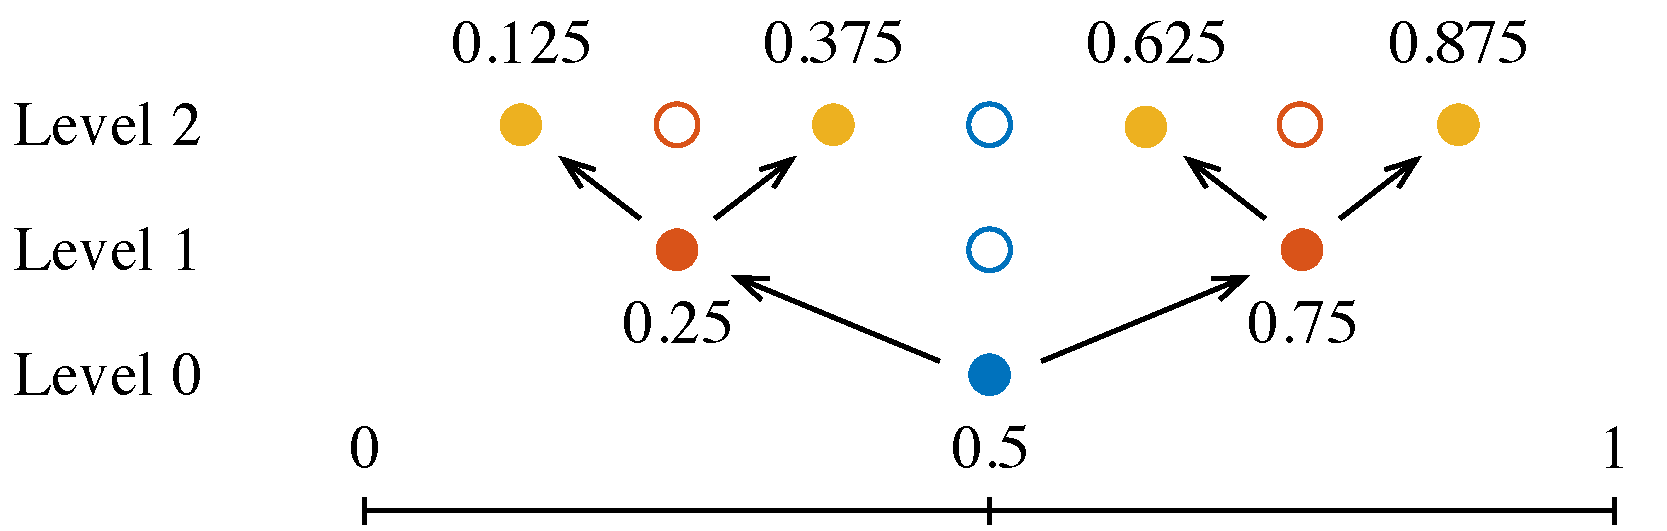
\includegraphics[width=1.0\columnwidth]{include/assets/rule.pdf}
  \caption{
    An illustration of the open Newton--Cotes rule on $[0, 1]$. On each level,
    the dots correspond to the nodes introduced by that particular level, and
    the wholes correspond to the nodes inherited from the previous levels.
  }
  \flab{rule}
\end{figure}

The open Newton--Cotes rule of level $i \in \natural$ is
\[
  \X^i = \left\{ x^i_j = \frac{j + 1}{\n_i + 1}: j \in \index(i) \right\}
\]
where $\index(i) = \left\{ 0, \dots, \n_i - 1 \right\}$ with $\n_i = 2^{i + 1} -
1$. The first three levels of the rule are depicted in \fref{rule}. It can be
seen that the number of nodes (in one dimension) grows as 1, 3, 7, 15, 31, and
so on, and the rule is fully nested. In multiple dimensions, the nodes are
formed as shown in \eref{collocation-nodes}.

\fref{rule} also illustrates the refinement strategies suitable for this grid.
The arrows emerging from a node connect the node with its next-level neighbors.
The number of such neighbors is two in one dimension and $2 \nin$ in general.
Formally, for a pair $(\vi, \vj)$, the neighbor pairs are
\[
  \left\{ \Big( (i_1, \dots, i_k + 1, \dots, i_\nin), (j_1, \dots, 2 j_k + c, \dots j_\nin) \Big) \right\}_{k, c}
\]
for $k = 1, \dots, \nin$ and $c \in \{ 0, 2 \}$. Whenever a node is to be
refined, some or all of its neighbors can be chosen for function evaluation. The
simplest strategy is to include all $2 \nin$ neighbors, which is what we shall
do.


\subsection{Basis Functions} \slab{basis-functions}
\begin{figure}[t]
  \centering
  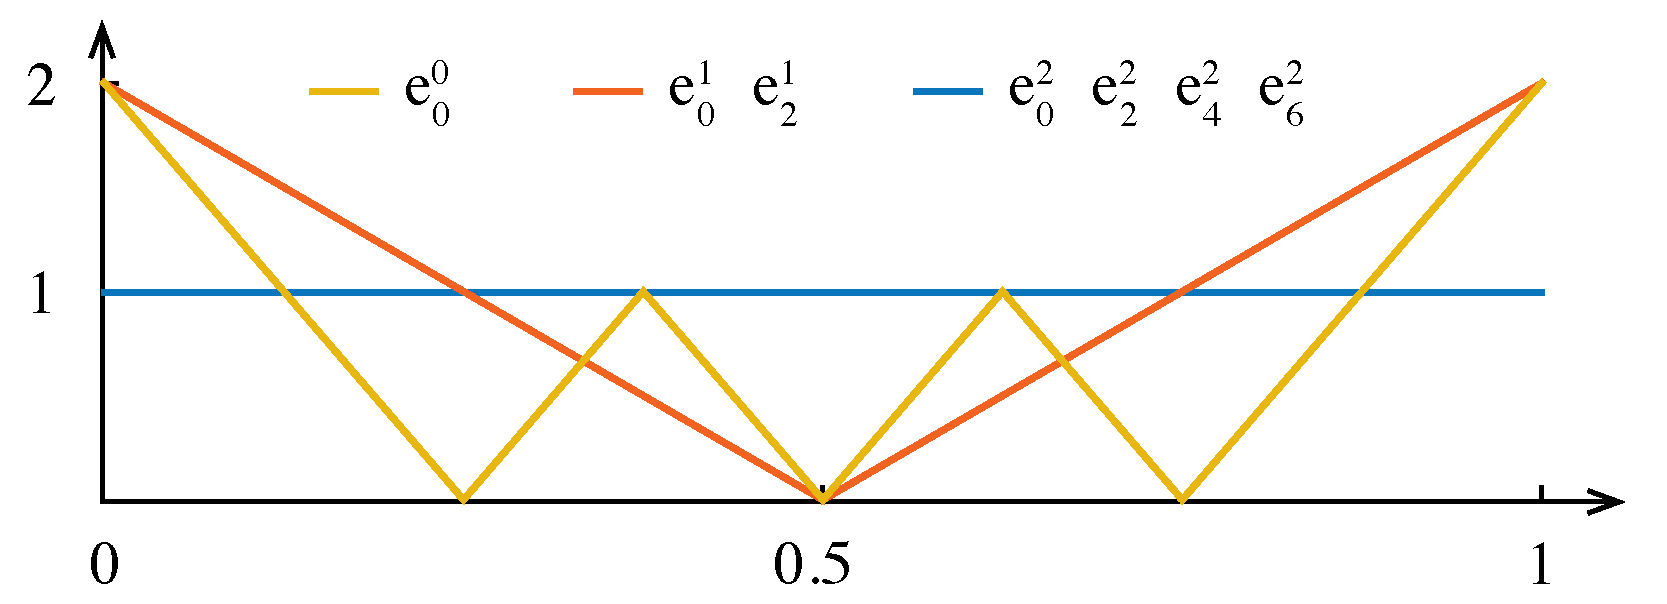
\includegraphics[width=1.0\columnwidth]{include/assets/figures/basis.pdf}
  \vspace{-1.5em}
  \caption{
    The first three levels of the basis described in \sref{basis}.
  }
  \flab{basis}
\end{figure}

The basis functions that go hand in hand with the open Newton--Cotes rule are
the following piecewise linear functions. For $i = 0$ and $j = 0$,
\[
  \e_{00}(\x) = 1.
\]
For $i > 0$ and $j = 0$ (close to the left endpoint),
\[
  \e_{i0}(\x) = \begin{cases}
    2 - \left( \n_i + 1 \right) \x, & \text{if } \x < \frac{2}{\n_i + 1}, \\
    0, & \text{otherwise}.
  \end{cases}
\]
For $i > 0$ and $j = \n_i - 1$ (close to the right endpoint),
\[
  \e_{i(\n_i - 1)}(\x) = \begin{cases}
    \left( \n_i + 1 \right) \x - \n_i + 1, & \text{if } \x > \frac{\n_i - 1}{\n_i + 1}, \\
    0, & \text{otherwise}.
  \end{cases}
\]
In other cases,
\[
  \e_{ij}(\x) = \begin{cases}
    1 - \left( \n_i + 1 \right)|\x - \x_{ij}|, & \text{if } |\x - \x_{ij}| < \frac{1}{\n_i + 1}, \\
    0, & \text{otherwise}.
  \end{cases}
\]
The basis functions corresponding to the first three levels of one-dimensional
interpolation are depicted in \fref{basis}. Note that $\e_{11}$, $\e_{21}$,
$\e_{23}$, and $\e_{25}$ are not depicted as they are not involved in the
hierarchical construction. In multiple dimensions, the basis functions are
formed as shown in \eref{basis-functions}.

Lastly, let us mention the volumes (integrals over the whole domain) of the
basis functions denoted by $\w_{ij}$; they will be needed in the future. Namely,
$\w_{00} = 1$ and, for $i > 0$,
\begin{equation} \elab{volume}
  \w_{ij} := \int_0^1 \e_{ij}(\x) \, \d\x = \begin{cases}
    \frac{2}{\n_i + 1}, & \text{if } j \in \{ 0, \n_i - 1 \}, \\
    \frac{1}{\n_i + 1}, & \text{otherwise}.
  \end{cases}
\end{equation}
In multiple dimensions, the volumes are products of the one-dimensional
components, analogous to \eref{basis-function}.

\begin{remark}
Instead of piecewise linear functions, one can also utilize locally supported
polynomials of higher orders \cite{jakeman2012}. However, we did not observe
much improvement and, therefore, do not discuss this alternative in the paper.
\end{remark}


\subsection{Implementation}
The life cycle of interpolation has roughly two stages: construction and usage.
The construction stage invokes $\f$ at a set of collocation nodes and produces
certain artifacts. The usage stage estimates the values of $\f$ at a set of
arbitrary points by manipulating the artifacts. In this subsection, we shall
look at the pseudocodes of the two stages. The purpose is to give the big
picture. A lot of implementation details are purposely omitted; however, all the
details can be found and studied online as our implementation is open source
\cite{sources}.

Let us first make a general note. We found it beneficial to the clarity and ease
of implementation to collapse the two sums in \eref{approximation} into one.
This requires storing a level index $\vi = (i_k)_{k = 1}^\nin$ and an order
index $\vj = (j_k)_{k = 1}^\nin$ for each interpolation element. It is also
advantageous to encode each pair $(i_k, j_k)$ as a single unsigned integer,
which, in particular, eliminates excessive memory usage. In multiple dimensions,
this results in a single vector $\vl = (\iota_k)_{k = 1}^\nin$, which we simply
call an index. The encoding that we utilize is as follows:
\[
  \iota_k = i_k \lor (j_k \ll \n_\text{bits})
\]
where $\lor$ and $\ll$ are the bitwise \up{OR} and logical left shift,
respectively, and $\n_\text{bits}$ is the number of bits reserved for storing
Smolyak levels, which can be adjusted according to the maximum permitted
deepness of interpolation.

The pseudocode of the construction stage is given in \aref{construct} called
\token{Construct}. The \token{target} input is a function $\f$ to be
approximated. The \token{surrogate} output is a structure containing the
artifacts of interpolation, which are a set of tuples $\{ (\vl_k,
\surplus(\vx_{\vl_k}) \}_k$, giving a comprehensive description of an
interpolant. The routine works as follows.

\begin{compactlist}

\point{Line~2:} Each iteration is an interpolation step in \eref{approximation}.
It has a state captured by a structure denoted by \token{s}. The
\token{strategy} object represents an adaptation strategy utilized and works as
described in \sref{adaptivity}. The \token{First} method of \token{strategy}
returns the initial state of the first step so that the \token{indices} field of
\token{s} is initialized with the indices of that step. The body of the loop
populates the rest of the fields of \token{s} so that \token{strategy.Next} can
adequately produce the initial state of the next iteration. The process
terminates when a stopping condition is satisfied, in which case \token{Next}
returns a null state.

\point{Line~3:} The \token{grid} object represents the interpolation grid
utilized (see \sref{grid}), and its \token{Compute} method converts the step's
indices into the coordinates of the corresponding collocation nodes, that is,
$\{ \vl_k \}_k$ into $\{ \vx_{\vl_k} \}_k$.

\point{Line~4:} \token{Invoke} evaluates \token{target} at the collocation
nodes. This is a prominent candidate for parallelization since the algorithm
does not impose any evaluation order; $\f$ can be calculated simultaneously for
all the nodes of the iteration.

\point{Line~5:} \token{Evaluate} exercises the interpolant constructed so far at
the collocation nodes, approximating the values obtained on line~4. This
function will be discussed separately.

\point{Line~6:} \token{Subtract} computes the difference between the true and
approximated values of \token{target}, which yields the step's hierarchical
surpluses $\{ \surplus(\vx_{\vl_k}) \}_k$, similar to \eref{surplus}.

\point{Line~7:} \token{strategy.Score} calculates the scores of the new
collocation nodes based on their surpluses; see \eref{score}.

\point{Line~8:} \token{Append} improves the interpolant by extending it with the
indices and surpluses of the current iteration.

\end{compactlist}

We now turn to the usage stage of an interpolant. The pseudocode is given in
\aref{evaluate} called \token{Evaluate}. This algorithm is also involved in
\aref{construct}; see line~5. Let us make a couple of observations regarding
\token{Evaluate}.

\begin{compactlist}

\point{Line~4:} The inner loop is an unfolded version of \eref{approximation}
(there is no separation between individual interpolation steps taken).

\point{Line~5:} The \token{basis} object represents the interpolation basis
utilized (see \sref{basis}), and its \token{Compute} method evaluates a single
(multidimensional) basis function at a single point.

\end{compactlist}

It is worth noting that the \token{basis}, \token{grid}, and \token{strategy}
objects conform to certain interfaces and can be easily swapped out. This makes
the two algorithms very general and reusable with different configurations. In
particular, the adaptation strategy can be fine-tuned for each particular
problem.



  \section{Analysis} \slab{analysis}
  In \sref{modeling}, we formalized the uncertainty affecting electronic systems
and introduced a number of models along with a number of quantities $\g$ that
the designer is typically interested in studying. In the previous section,
\sref{interpolation}, we obtained an efficient interpolation algorithm for
approximating hypothetical multidimensional functions $\f$. Now we shall
amalgamate the ideas developed in the aforementioned two sections.

Given an electronic system dependent on a number of uncertain parameters $\vu:
\outcomes \to \real^\nu$, the goal is to analyze a quantity of interest $\g$
representing a certain aspect of the system. For instance, $\vu$ can correspond
to the execution times of the tasks that the processing elements are to execute,
and $\g$ can correspond the total energy consumed by the processing elements.
The goal is attained as follows. First, the parametrization of $\g$ is changed
from $\vu$ to \rvs\ $\vz: \outcomes \to [0, 1]^\nz$ via a suitable
transformation $\transformation$; this stage is described in \sref{parameters}.
Second, an interpolant of the resulting composition $\g \circ \transformation$
is constructed by treating the composition as a deterministic function $\f$ of
$\vz$; this stage is detailed in \sref{interpolation}. Third, an estimation of
the probability distribution of $\g$ is undertaken in the usual sampling-based
manner but relying solely on the constructed interpolant; $\g$ is no longer
involved. This last stage boils down to drawing independent samples from
$\distribution_\vz$ and evaluating the interpolant $\approximation{\l}(\f)
\equiv \approximation{\l}(\g \circ \transformation)$ at those points. Needless
to say that, having collected samples of $\g$, other statistics about $\g$, such
as probabilities of particular events, can be straightforwardly estimated. We do
not discuss the estimation stage any further as it is standard. However, there
are two other aspects concerning the usage of the proposed framework that we
would like to cover in what follows.

\subsection{Expectation and Variance} \slab{probabilistic-moments}
Since the expected value and variance, defined in \eref{expectation} and
\eref{variance}, respectively, usually draw particular attention, we would like
to elaborate on them separately; the interpolants that we construct have
something special to offer in this regard.

As shown in \sref{parameters}, $\g$ can be reparameterized in terms of
independent variables that are uniformly distributed on $[0, 1]^\nz$. This means
that the probability density function of $\vz$ simply equals to one. Therefore,
by the law of the unconscious statistician, using \eref{expectation} and
\eref{approximation}, we have
\begin{align*}
  \expectation{\g} \approx \expectation{\approximation{\l}(\f)} &= \int_{[0, 1]^\nz} \approximation{\l}(\f)(\vz) \, \d\vz \\
  &= \sum_{\vi \in \lindex_\l} \, \sum_{\vj \in \Delta\oindex_\vi} \surplus(\vx_{\vi\vj}) \, \w_{\vi\vj}
\end{align*}
where
\[
  \w_{\vi\vj} = \int_{[0, 1]^\nz} \e_{\vi\vj}(\vz) \, \d\vz = \prod_{k = 1}^{\nz} \int_0^1 \e_{i_k j_k}(\z_k) \, \d\z_k = \prod_{k = 1}^{\nz} \w_{i_k j_k}.
\]
In the above equation, $\w_{ij}$ is as shown in \eref{volume}. Consequently, we
have obtained an analytical formula for the expected value of $\g$, which does
not require any sampling.

Regarding the variance of $\g$, it can be seen in \eref{variance} that the
variance can be assembled from two components: the expected value of $\g$, which
we already have, and the expected value of $\g^2$, which we are missing. The
solution is to let $h = (\g, \g^2)$ be the quantity of interest instead of $\g$.
Then the expected values of both $\g$ and $\g^2$ will be available in analytical
forms, and the variance of $\g$ can be computed using \eref{variance}. This
approach can be generalized to probabilistic moments of higher orders.

\subsection{Multiple Outputs}
The careful reader has noted a problem with the calculation of variance in the
previous subsection: $h$ is vector valued. More generally, the quantity $\g$ in
\sref{modeling} and the function $\f$ in \sref{interpolation} have been depicted
so far as having one-dimensional codomains. This, however, has been done only
for the sake of clarity. All the mathematics and pseudocodes stay the same for
vector-valued functions. The only except is that, since a surplus
$\surplus(\vx_{\vi\vj})$ naturally inherits the output dimensionality of $\f$,
the operations that involve $\surplus(\vx_{\vi\vj})$ should be adequately
adjusted. If the outputs are on different scales and/or have different accuracy
requirements, one might want to have different $\aerror$ and $\rerror$ in
\eref{stopping-condition} for different outputs. In that case, one also need to
device a more sensible strategy for scoring collocation nodes in \eref{score}
such as rescaling individual outputs and then calculating the uniform norm
$\norm{\cdot}_\infty$ or $L^2$ norm $\norm{\cdot}_2$. Our code \cite{sources}
has been written with multiple outputs in mind.

To sum up, once an interpolant of $\g$ has been constructed, the distribution of
$\g$ is estimated using versatile sampling methods applied to the interpolant.
The framework extends naturally to quantities of interest with multiple outputs,
and it provides analytical formulae for expectations and variances.


  \section{Experimental Results} \slab{experimental-results}
  In this section, we evaluate the performance of the proposed framework. Our
prototype of the framework had been implemented in the Go programming language
\cite{go}. The prototype is divided into multiple independent packages, and the
corresponding source codes are available online \cite{sources}. The source code
of the experimental setup below along with the input data are also available at
\cite{sources}. The experiments are conducted on a \abbr{GNU}/Linux machine
equipped with 16 processors Intel Xeon E5520 2.27~\abbr{GH}z and 24~\abbr{GB} of
\abbr{RAM}.

Each problem that we consider is structured as follow. A platform $\procs$ with
$\np$ processing elements and an application $\tasks$ with $\nt$ tasks are
generated randomly by the \abbr{TGFF} tool \cite{dick1998}. The tool generates
$\np$ tables and a directed acyclic graph with $\nt$ nodes. Each table
corresponds to a processing element, and it describes certain properties of the
tasks when they are mapped to that particular processing element. Namely, each
table assigns two numbers to each task: a reference execution time, chosen
uniformly between 10 and 50~ms, and a power consumption, chosen uniformly
between 5 and 15~W. The graph captures data dependencies between the tasks. The
application is scheduled using a list scheduler \cite{adam1974}. The mapping of
the application is fixed and obtained by scheduling the tasks based on their
reference execution times and assigning them to the earliest available
processing elements (a shared ready list).

The construction of thermal \abbr{RC} circuits needed for temperature analysis
is delegated to the HotSpot tool \cite{skadron2004}. The floorplan of each
platform is a regular grid wherein each processing element occupies $2 \times
2~\text{mm}^2$ on the die. The output of the tool is essentially a pair of a
thermal capacitance matrix $\mC$ and a thermal conductance $\mG$ matrix used in
\eref{thermal-system}. The leakage modeling is based on a linear approximation
\cite{yang2013, ukhov2012, liu2007}.

\begin{figure}[t]
  \centering
  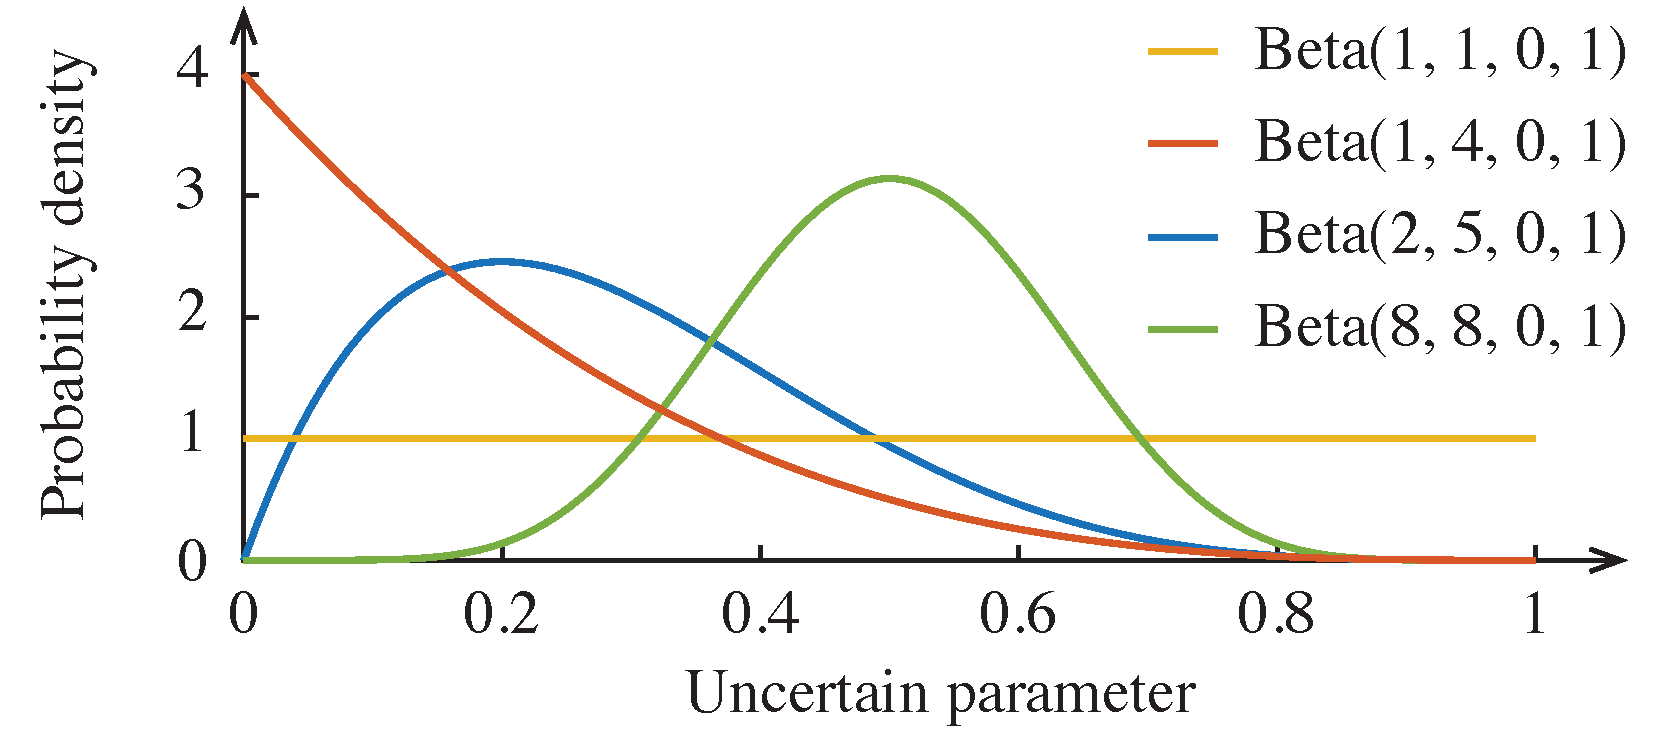
\includegraphics[width=1.0\columnwidth]{include/assets/figures/distribution.pdf}
  \caption{An illustration of the family of beta distributions.}
  \flab{distribution}
\end{figure}

The uncertain parameters $\vu$ are the execution times of the tasks; all other
parameters are deterministic. Targeting the practical scenario described in
\sref{uncertain-parameters}, the marginal distributions and correlation matrix
of $\vu$ are assumed to be available. Without loss of generality, the marginal
of $\u_i$ is a four-parametric beta distribution $\text{Beta}(\alpha_i, \beta_i,
a_i, b_i)$ where $\alpha_i$ and $\beta_i$ are the shape parameters, and $a_i$
and $b_i$ are the endpoints of the support. This family of distributions is very
reach; \fref{distribution} illustrates how the density function changes
dramatically depending on $\alpha_i$ and $\beta_i$. The left endpoint $a_i$ is
set to the reference execution time generated by the \abbr{TGFF} tool as
discussed earlier, and the right endpoint $b_i$ is set to be 20\% larger than
$a_i$. The parameters $\alpha_i$ and $\beta_i$ are set to two and five,
respectively, for all tasks, skewing their uncertain execution times towards the
reference execution times (the blue curve in \fref{distribution}). The execution
times of the tasks are correlated based on the structure of the graph produced
by the \abbr{TGFF} tool: the closer the $i$th and $j$th tasks are in the graph
as measured by the number of edges between the $i$th and $j$th nodes, the
stronger $\u_i$ and $\u_j$ are correlated.

Regarding the interpolation algorithm, we rely on the open Newton--Cotes rule as
motivated in \sref{collocation-nodes}. The \token{IsEnough} subroutine of
\aref{construct} terminates the algorithm when it reaches a certain
interpolation level. The decision taken in \token{IsAccurate} is based on the
formula given in \eref{error}.

Lastly, we would like to remind that our setup is publicly available
\cite{sources}. The configuration aspects that have not been explicitly
mentioned here, such as the configuration files of the \abbr{TGFF} and HotSpot
tools, can be found online.

The quantities of interest $\g$ that we shall consider are: 1) the end-to-end
delay of the application, 2) the total energy consumed by the system, and 3) a
temperature profile of the system, which are given by \eref{end-to-end-delay},
\eref{total-energy}, and \eref{temperature-profile}, respectively.

\subsection{End-to-End Delay}
\begin{table*}
  \caption{End-to-end delay}
  \begin{tabular*}{\textwidth}{=R{10pt}-R{25pt}-R{50pt}-R{25pt}-R{50pt}-R{25pt}-R{50pt}-R{25pt}-R{50pt}-R{25pt}-R{50pt}}
    \toprule
    & \multicolumn{2}{c}{2/20} & \multicolumn{2}{c}{4/40} & \multicolumn{2}{c}{8/80} & \multicolumn{2}{c}{16/160} & \multicolumn{2}{c}{32/320} \\
    \cmidrule( r){1-1}
    \cmidrule(l ){2-3}
    \cmidrule(l ){4-5}
    \cmidrule(l ){6-7}
    \cmidrule(l ){8-9}
    \cmidrule(l ){10-11}
     2 &  31 & $2.69 \times 10^{-2}$ &  67 & $2.64 \times 10^{-2}$ & 119 & $2.83 \times 10^{-2}$ & 187 & $2.82 \times 10^{-2}$ &  965 & $2.62 \times 10^{-2}$ \\
     4 &  67 & $1.12 \times 10^{-2}$ & 176 & $1.05 \times 10^{-2}$ & 245 & $1.24 \times 10^{-2}$ & 531 & $1.78 \times 10^{-2}$ & 2207 & $1.37 \times 10^{-2}$ \\
     6 &  85 & $5.88 \times 10^{-3}$ & 236 & $5.85 \times 10^{-3}$ & 315 & $7.56 \times 10^{-3}$ & 692 & $1.29 \times 10^{-2}$ & 2795 & $1.02 \times 10^{-2}$ \\
     8 &  97 & $4.29 \times 10^{-3}$ & 256 & $5.26 \times 10^{-3}$ & 343 & $6.84 \times 10^{-3}$ & 728 & $1.28 \times 10^{-2}$ & 3089 & $9.48 \times 10^{-3}$ \\
    10 & 109 & $3.84 \times 10^{-3}$ & 276 & $5.22 \times 10^{-3}$ & 371 & $6.78 \times 10^{-3}$ & 764 & $1.28 \times 10^{-2}$ & 3257 & $9.34 \times 10^{-3}$ \\
    \bottomrule
  \end{tabular*}
  \tlab{end-to-end-delay}
\end{table*}
% vim: nowrap tw=0

The quantity of interest $\g$ considered in this subsection is the end-to-end
delay given in \eref{end-to-end-delay}, which is a scalar.

\subsection{Total Energy}
\begin{table*}
  \caption{Total energy}
  \begin{tabular*}{\textwidth}{=R{10pt}-R{25pt}-L{50pt}-R{25pt}-L{50pt}-R{25pt}-L{50pt}-R{25pt}-L{50pt}-R{25pt}-L{50pt}}
    \toprule
    & \multicolumn{2}{c}{1/10} & \multicolumn{2}{c}{4/40} & \multicolumn{2}{c}{9/90} & \multicolumn{2}{c}{16/160} & \multicolumn{2}{c}{25/250} \\
    \cmidrule( r){1-1}
    \cmidrule(l ){2-3}
    \cmidrule(l ){4-5}
    \cmidrule(l ){6-7}
    \cmidrule(l ){8-9}
    \cmidrule(l ){10-11}
     2 & 0 & $0.00 \times 10^{-0}$ & 0 & $0.00 \times 10^{-0}$ & 0 & $0.00 \times 10^{-0}$ & 0 & $0.00 \times 10^{-0}$ & 0 & $0.00 \times 10^{-0}$ \\
     4 & 0 & $0.00 \times 10^{-0}$ & 0 & $0.00 \times 10^{-0}$ & 0 & $0.00 \times 10^{-0}$ & 0 & $0.00 \times 10^{-0}$ & 0 & $0.00 \times 10^{-0}$ \\
     6 & 0 & $0.00 \times 10^{-0}$ & 0 & $0.00 \times 10^{-0}$ & 0 & $0.00 \times 10^{-0}$ & 0 & $0.00 \times 10^{-0}$ & 0 & $0.00 \times 10^{-0}$ \\
     8 & 0 & $0.00 \times 10^{-0}$ & 0 & $0.00 \times 10^{-0}$ & 0 & $0.00 \times 10^{-0}$ & 0 & $0.00 \times 10^{-0}$ & 0 & $0.00 \times 10^{-0}$ \\
    10 & 0 & $0.00 \times 10^{-0}$ & 0 & $0.00 \times 10^{-0}$ & 0 & $0.00 \times 10^{-0}$ & 0 & $0.00 \times 10^{-0}$ & 0 & $0.00 \times 10^{-0}$ \\
    \bottomrule
  \end{tabular*}
  \tlab{total-energy}
\end{table*}
% vim: nowrap tw=0

Let the quantity of interest $\g$ be the total energy given in
\eref{total-energy}, which is a scalar.

\subsection{Temperature Profile}
\begin{table*}
  \caption{Temperature profile}
  \begin{tabular*}{\textwidth}{=R{10pt}-R{25pt}-R{50pt}-R{25pt}-R{50pt}-R{25pt}-R{50pt}-R{25pt}-R{50pt}-R{25pt}-R{50pt}}
    \toprule
    & \multicolumn{2}{c}{2/20} & \multicolumn{2}{c}{4/40} & \multicolumn{2}{c}{8/80} & \multicolumn{2}{c}{16/160} & \multicolumn{2}{c}{32/320} \\
    \cmidrule( r){1-1}
    \cmidrule(l ){2-3}
    \cmidrule(l ){4-5}
    \cmidrule(l ){6-7}
    \cmidrule(l ){8-9}
    \cmidrule(l ){10-11}
     2 & 0 & $0.00 \times 10^{-0}$ & 0 & $0.00 \times 10^{-0}$ & 0 & $0.00 \times 10^{-0}$ & 0 & $0.00 \times 10^{-0}$ & 0 & $0.00 \times 10^{-0}$ \\
     4 & 0 & $0.00 \times 10^{-0}$ & 0 & $0.00 \times 10^{-0}$ & 0 & $0.00 \times 10^{-0}$ & 0 & $0.00 \times 10^{-0}$ & 0 & $0.00 \times 10^{-0}$ \\
     6 & 0 & $0.00 \times 10^{-0}$ & 0 & $0.00 \times 10^{-0}$ & 0 & $0.00 \times 10^{-0}$ & 0 & $0.00 \times 10^{-0}$ & 0 & $0.00 \times 10^{-0}$ \\
     8 & 0 & $0.00 \times 10^{-0}$ & 0 & $0.00 \times 10^{-0}$ & 0 & $0.00 \times 10^{-0}$ & 0 & $0.00 \times 10^{-0}$ & 0 & $0.00 \times 10^{-0}$ \\
    10 & 0 & $0.00 \times 10^{-0}$ & 0 & $0.00 \times 10^{-0}$ & 0 & $0.00 \times 10^{-0}$ & 0 & $0.00 \times 10^{-0}$ & 0 & $0.00 \times 10^{-0}$ \\
    \bottomrule
  \end{tabular*}
  \tlab{temperature-profile}
\end{table*}
% vim: nowrap tw=0

In this subsection, the quantity of interest $\g$ is the temperature profile
$\mQ$ of the system calculated using \eref{thermal-system}. The profile is an
$\np \times \ns$ matrix, and, therefore, $\g$ is $\np \ns$-dimensional.


  \section{Conclusion} \slab{conclusion}
  In this paper, we have presented a framework for probabilistic analysis of
electronic systems. Given a description of the probability distribution of the
uncertain parameters present in the system under consideration and a simulator
of a metric of interest dependent on the parameters, the framework prescribes
the steps that need to be taken in order to computationally efficiently obtain
the probability distribution of the metric.

The proposed approach is powered by hierarchical interpolation following a
hybrid adaptation strategy. The adaptivity makes the framework particularly
suited for problems with idiosyncratic behaviors and steep response surfaces,
which arise in electronic systems due to their digital nature.

The performance of our framework has been assessed by comparing it with the
performance of an advanced sampling technique. The experimental results have
shown that, for a fixed budget of evaluations of the metric, our approach
achieves higher accuracy compared to direct simulations.

Finally, we would like to emphasize that, even though the framework has been
exemplified by considering a specific source of uncertainty and specific
metrics, it is general and can be successfully applied in many other settings.


  \section*{Acknowledgments}
  The authors would like to thank Prof. Nicholas Zabaras and Dr. Xiang Ma from
Cornell University and Dr. Stefan Dirnstorfer from Munich Technical University
for the help with adaptive hierarchical interpolation and integration
techniques.


  \begingroup
    \bibliographystyle{IEEEtran}
    \bibliography{IEEEabrv,include/references}
  \endgroup
\end{document}
